\documentclass[a4paper]{amsart}

\usepackage[greek,english]{babel}
\usepackage{microtype}

\usepackage[T1]{fontenc}
\usepackage{libertinus}
\usepackage{amsmath}
\usepackage{amssymb}
\usepackage{mathtools}

\usepackage[
  libertinus,
  noto,
  vvarbb,
  amsthm,
]{newtx}

\usepackage{xfrac}
\usepackage{xcolor}

\usepackage{tikz}
\usetikzlibrary{arrows}
\usetikzlibrary{arrows.meta}

\usepackage[pdftex,
            pdfauthor={Michael Eisermann},
            pdftitle={Formalizing Pick's Theorem in Lean},
            pdfstartview=FitH,
            colorlinks=true,
            anchorcolor=black, 
            linkcolor=black, 
            urlcolor=black,
            citecolor=black, 
            pagecolor=black, 
            filecolor=black, 
            menucolor=black, 
            ]{hyperref}

\usepackage[a4paper]{geometry}
\geometry{
  width=135mm,
  height=240mm,
  headsep=5mm,
  footskip=20mm,
}

\title{Formalizing Pick's Theorem in Lean}

\author{Elli zu Neblberg}

\address{Institut für Geometrie und Topologie, Universität Stuttgart, Germany}
\email{Michael.Eisermann@mathematik.uni-stuttgart.de}
% \urladdr{www.igt.uni-stuttgart.de/eiserm}

\date{first version September 2024; this version compiled \today}

%%%%%%%%%%%%%%%%%%%%%%%%%%%%%%%%%%%%%%%%%%%%%%%%%%%%%%%%%%%%%%%%%%%%%%%%%%%%%
%%% theorem environments %%%%%%%%%%%%%%%%%%%%%%%%%%%%%%%%%%%%%%%%%%%%%%%%%%%%
%%%%%%%%%%%%%%%%%%%%%%%%%%%%%%%%%%%%%%%%%%%%%%%%%%%%%%%%%%%%%%%%%%%%%%%%%%%%%

\numberwithin{equation}{section}

\theoremstyle{plain}
  \newtheorem{theorem}{Theorem}[section]
  \newtheorem{lemma}[theorem]{Lemma}
  \newtheorem{proposition}[theorem]{Proposition}
  \newtheorem{corollary}[theorem]{Corollary}
  
\theoremstyle{definition}
  \newtheorem{definition}[theorem]{Definition}
  \newtheorem{assumption}[theorem]{Assumption}
  \newtheorem{question}[theorem]{Question}
  \newtheorem{conjecture}[theorem]{Conjecture}
  \newtheorem{remark}[theorem]{Remark}
  \newtheorem{example}[theorem]{Example}
  
%%%%%%%%%%%%%%%%%%%%%%%%%%%%%%%%%%%%%%%%%%%%%%%%%%%%%%%%%%%%%%%%%%%%%%%%%%%%%  
%%% frequently used mathematical symbols %%%%%%%%%%%%%%%%%%%%%%%%%%%%%%%%%%%%
%%%%%%%%%%%%%%%%%%%%%%%%%%%%%%%%%%%%%%%%%%%%%%%%%%%%%%%%%%%%%%%%%%%%%%%%%%%%%

\newcommand{\N}{\mathbb{N}}
\newcommand{\Z}{\mathbb{Z}}
\newcommand{\Q}{\mathbb{Q}}
\newcommand{\R}{\mathbb{R}}
\newcommand{\K}{\mathbb{K}}

\newcommand{\ii}[2]{\mathopen[ #1, #2 \mathclose]}
\newcommand{\ie}[2]{\mathopen[ #1, #2 \mathclose[}
\newcommand{\ei}[2]{\mathopen] #1, #2 \mathclose]}
\newcommand{\ee}[2]{\mathopen] #1, #2 \mathclose[}

\newcommand{\fade}{\color{black!50}}
\newcommand{\dark}{\color{black}}

\newcommand{\minus}{\smallsetminus}
\newcommand{\abs}[1]{\lvert #1 \rvert}
\newcommand{\bigabs}[1]{\bigl\lvert #1 \bigr\rvert{}}

\DeclareMathOperator{\sign}{sign}
\DeclareMathOperator{\vol}{vol}
\DeclareMathOperator{\supp}{supp}

\newcommand{\area}{\mathrm{area}}
\newcommand{\Area}{\mathrm{Area}}
\newcommand{\ang}{\mathrm{ang}}
\newcommand{\Ang}{\mathrm{Ang}}
\newcommand{\dang}{\mathrm{dang}}
\newcommand{\Dang}{\mathrm{Dang}}
\newcommand{\welp}{\mathrm{welp}}
\newcommand{\Welp}{\mathrm{Welp}}

% \renewcommand{\Colon}{\nobreak\mskip+2mu\mathrel{:}\mskip+2mu\relax}

\def\middlevert{\mskip-0mu\mid\mskip-0mu}
\begingroup
\catcode`\|=\active
\gdef\set#1{\begingroup \mathcode`\|32768 \let|\middlevert \{\mskip2mu #1 \mskip2mu\} \endgroup}
\endgroup

%%%%%%%%%%%%%%%%%%%%%%%%%%%%%%%%%%%%%%%%%%%%%%%%%%%%%%%%%%%%%%%%%%%%%%%%%%%%%
\begin{document} %%%%%%%%%%%%%%%%%%%%%%%%%%%%%%%%%%%%%%%%%%%%%%%%%%%%%%%%%%%%
%%%%%%%%%%%%%%%%%%%%%%%%%%%%%%%%%%%%%%%%%%%%%%%%%%%%%%%%%%%%%%%%%%%%%%%%%%%%%

\begin{abstract}
  Pick's astonishing theorem explains how to obtain % says that we obtain % can calculate
  the area of any integer polygon by counting lattice points. % suitably
  % Traditional proofs intend to convince humans % are intended for human understanding
  % and are thus optimized for visual intuition. % therefore typically 
  It is a notorious challenge % difficult % tricky
  to translate the geometric statement and intuitive reasoning
  into a formal statement and rigorous proof. %, suitable for a proof assistant. % like Lean. 
  % Our approach is thus twofold:
  We transform the beautiful geometry into equally elegant algebra,
  and then implement the algebraic proof in Lean.  
\end{abstract}

\maketitle

%%%%%%%%%%%%%%%%%%%%%%%%%%%%%%%%%%%%%%%%%%%%%%%%%%%%%%%%%%%%%%%%%%%%%%%%%%%%%

\section{Introduction} \label{sec:Introduction}

\bibliographystyle{amsplain}
\bibliography{leanpick}

A \emph{polygon} $P = (p_0,p_1,\ldots,p_n)$ is % given by
a finite sequence of points $p_i = (x_i,y_i) \in \R^2$.
It defines the corresponding path $\gamma \colon [0,1] \to \R^2$
by piecewise linear interpolation of the given vertices
$\gamma(i/n) = p_i$ for $i=0,1,\dots,n$.
We call $P$ \emph{closed} if $p_0 = p_n$, and
\emph{simply closed} if $\gamma(s) = \gamma(t)$
only holds for $s = t$ or $\{s,t\} = \{0,1\}$.
In this case Jordan's theorem applies:
The polygonal curve $C = \gamma([0,1]) \subset \R^2$
separates the plane in two connected open sets $A$ and $B$,
so $\R^2 = A \sqcup B \sqcup C$, where the \emph{exterior region} $A$
is unbounded and the \emph{interior region} $B$ is bounded.
Their common boundary is the curve $C$, so their closures
are $\bar{A} = A \cup C$ and $\bar{B} = B \cup C$.

\begin{figure}[ht]
  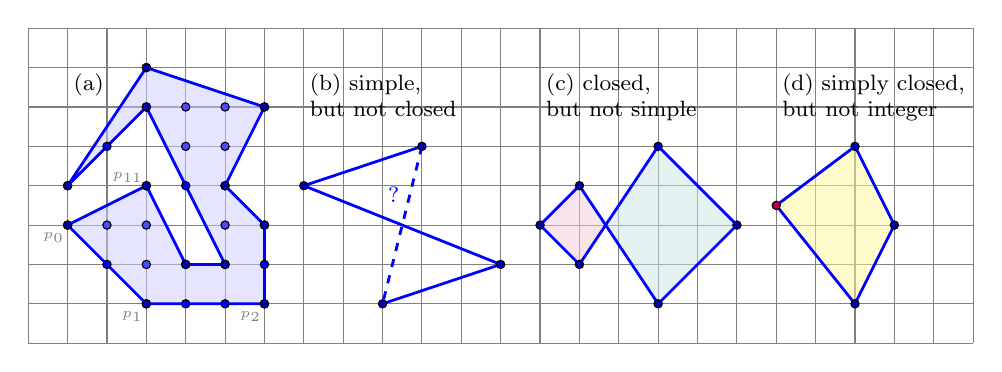
\begin{tikzpicture}[x=5mm, y=5mm, font=\footnotesize,
      rounded corners=0.2pt, inner sep=2pt, align= left]
    \setlength{\baselineskip}{5mm}
    \draw[color=black!50, step=1] (-1,-1) grid (23,7);
    \begin{scope}[shift={(0,0)}]
      \draw[line width=1pt, blue, fill=blue!20, fill opacity=0.5]
      (0,2) -- (2,0) -- (5,0) -- (5,2) -- (4,3) -- (5,5) --
      (2,6) -- (0,3) -- (2,5) -- (4,1) -- (3,1) -- (2,3) -- cycle;
      \draw[inner sep=1pt, font=\tiny\fade\mathstrut] 
      (2,3) node[above left]{$p_{11}$}
      (0,2) node[below left]{$p_0$}
      (2,0) node[below left]{$p_1$}
      (5,0) node[below left]{$p_{2}$};
      \foreach \x/\y in { 1/2, 2/1, 2/2, 3/4, 3/5, 4/2, 4/4, 4/5 }{
        \draw[draw=black, thin, fill=blue!70!white] (\x,\y) circle[radius=1.5pt];
      }
      \foreach \x/\y in { 0/2, 1/1, 2/0, 3/0, 4/0, 5/0, 5/1, 5/2,
        4/3, 5/5, 2/6, 0/3, 1/4, 2/5, 3/3, 4/1, 3/1, 2/3 }{
        \draw[draw=black, thin, fill=blue] (\x,\y) circle[radius=1.5pt];
      }
      \foreach \x/\y in { 0/2, 2/0, 5/0, 5/2, 4/3, 5/5, 2/6, 0/3, 2/5, 4/1, 3/1, 2/3 }{
        \draw[draw=black, thin, fill=blue!70!black] (\x,\y) circle[radius=1.5pt];
      }
      \draw (0,6) node[below right] {(a)};
    \end{scope}
    \begin{scope}[shift={(6,0)}]
      \draw (0,6) node[below right]{(b) simple, \\ but not closed};
      % (b) einfach, aber \\ nicht geschlossen};
      \draw[line width=1pt, blue] (2,0) -- (5,1) -- (0,3) -- (3,4);
      \draw[line width=1pt, blue, dashed ] (3,4) -- (2,0) node[pos=0.4, above left]{?};
      \foreach \x/\y in { 2/0, 5/1, 0/3, 3/4 }{
        \draw[draw=black, thin, fill=blue!70!black] (\x,\y) circle[radius=1.5pt];
      }      
    \end{scope}
    \begin{scope}[shift={(12,0)}]
      \draw (0,6) node[below right]{(c) closed, \\ but not simple};
      % (c) geschlossen, \\ aber nicht einfach};
      \draw[draw=none, fill=purple!20, fill opacity=0.5]
      (0,2) -- (1,1) -- (5/3,2) -- (1,3) -- cycle;
      \draw[draw=none, fill=teal!20, fill opacity=0.5]
      (5/3,2) -- (3,4) -- (5,2) -- (3,0) -- cycle;
      \draw[line width=1pt, blue]
      (0,2) -- (1,1) -- (3,4) -- (5,2) -- (3,0) -- (1,3) -- cycle;
      \foreach \x/\y in { 0/2, 1/1, 3/4, 5/2, 3/0, 1/3 }{
        \draw[draw=black, thin, fill=blue!70!black] (\x,\y) circle[radius=1.5pt];
      }
    \end{scope}
    \begin{scope}[shift={(18,0)}]
      \draw (0,6) node[below right, ]{(d) simply closed, \\ but not integer};
      % {(d) nicht \\ ganzzahlig};
      \draw[line width=1pt, blue, fill=yellow!40, fill opacity=0.5]
      (0,2.5) -- (2,0) -- (3,2) -- (2,4) -- cycle;
      \foreach \x/\y in { 2/0, 3/2, 2/4 }{
        \draw[draw=black, thin, fill=blue!70!black] (\x,\y) circle[radius=1.5pt];
      }
      \draw[draw=black, thin, fill=purple] (0.0,2.5) circle[radius=1.5pt];
    \end{scope}
  \end{tikzpicture}
\end{figure}

Let $\vol_2(B)$ denote the enclosed area.
On the other hand, we can count the number of lattice points,
$I := \abs{ \Z^2 \cap B }$ in the interior and
$J := \abs{ \Z^2 \cap C }$ on the boundary $C = \partial B = \partial A$.

Here the magic of Pick's theorem happens:

\begin{theorem}[Georg Pick 1899] \label{thm:PickCombinatorial}
  Let $P = (p_0,p_1,\ldots,p_n=p_0)$
  be a simply closed polygon with integer vertices $p_i \in \Z^2$.
  Then $\vol_2(B) = I + J/2 - 1$.
\end{theorem}

\begin{figure}[ht]
  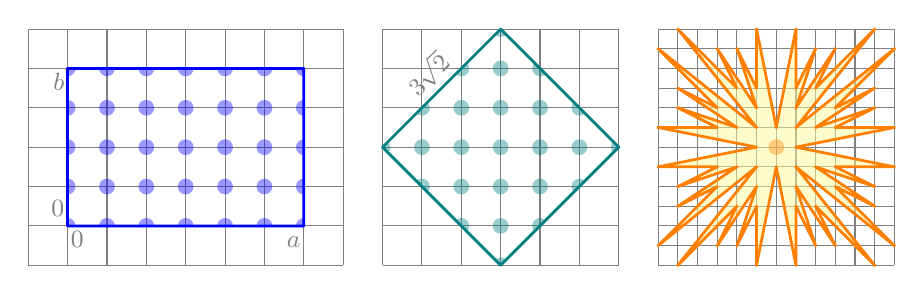
\begin{tikzpicture}[x=5mm, y=5mm, rounded corners=0.1pt]
    \begin{scope}[shift={(-5,-2)}]
      \draw[color=black!50, step=1] (-1,-1) grid (7,5);
      \draw[line width=1pt, blue] (0,0) rectangle (6,4);
      \draw[inner sep=1pt, font=\small\fade\mathstrut] 
      (0,0) node[below right]{$0$}
      (6,0) node[below left]{$a$}
      (0,0) node[above left]{$0$}
      (0,4) node[below left]{$b$};
      \clip (0,0) rectangle (6,4);
      \foreach \x in {0,...,6}{
        \foreach \y in {0,...,4}{
          \draw[draw=none, fill=blue, fill opacity=0.4] (\x,\y) circle[radius=1mm];
        }
      }
    \end{scope}
    \begin{scope}[shift={(6,0)}]
      \draw[color=black!50, step=1] (-3,-3) grid (3,3);
      \draw[line width=1pt, teal] (+3,0) -- (0,+3) -- (-3,0) -- (0,-3) -- cycle;
      \draw[draw=none, inner sep=1pt, font=\small\fade\mathstrut]
      (-3,0) -- (0,+3) node[midway, sloped, above] {$3\sqrt{2}$}; 
      \clip (+3,0) -- (0,+3) -- (-3,0) -- (0,-3) -- cycle;
      \foreach \x in {-3,...,3}{
        \foreach \y in {-3,...,3}{
          \draw[draw=none, fill=teal, fill opacity=0.4] (\x,\y) circle[radius=1mm];
        }
      }
    \end{scope}
    \begin{scope}[shift={(13,0)}, x=2.5mm, y=2.5mm]
      \draw[color=black!50, step=1] (-6,-6) grid (6,6); % (-7,-7) grid (7,7);
      \draw[line width=1pt, orange, fill=yellow!40, fill opacity=0.5]
      (+1,+0) -- (+6,+1) -- (+3,+1) -- (+5,+2) -- (+2,+1) -- (+5,+3) -- (+3,+2) -- (+6,+5) --
      (+1,+1) -- (+5,+6) -- (+2,+3) -- (+3,+5) -- (+1,+2) -- (+2,+5) -- (+1,+3) -- (+1,+6) --
      (-0,+1) -- (-1,+6) -- (-1,+3) -- (-2,+5) -- (-1,+2) -- (-3,+5) -- (-2,+3) -- (-5,+6) --
      (-1,+1) -- (-6,+5) -- (-3,+2) -- (-5,+3) -- (-2,+1) -- (-5,+2) -- (-3,+1) -- (-6,+1) --
      (-1,-0) -- (-6,-1) -- (-3,-1) -- (-5,-2) -- (-2,-1) -- (-5,-3) -- (-3,-2) -- (-6,-5) --
      (-1,-1) -- (-5,-6) -- (-2,-3) -- (-3,-5) -- (-1,-2) -- (-2,-5) -- (-1,-3) -- (-1,-6) --
      (+0,-1) -- (+1,-6) -- (+1,-3) -- (+2,-5) -- (+1,-2) -- (+3,-5) -- (+2,-3) -- (+5,-6) --
      (+1,-1) -- (+6,-5) -- (+3,-2) -- (+5,-3) -- (+2,-1) -- (+5,-2) -- (+3,-1) -- (+6,-1) --
      cycle;
      \draw[draw=none, fill=orange, fill opacity=0.4] (0,0) circle[radius=1mm];
    \end{scope}
  \end{tikzpicture}
  \caption{(a) rectangle, (b) oblique square, (c) Farey sunburst $F_6$}
  \label{fig:PickExamples}
\end{figure}

\begin{example}
  (a) As a simple illustration, consider % any integer rectangle
  the rectangle $R = [0,a] \times [0,b]$ with $a,b \in \N_{\ge1}$.
  We find $I = (a-1) (b-1)$ and $J = 2 a + 2 b$,
  which nicely adds up to $\vol_2(R) = a b$.

  (b) For the oblique square $Q$ of \autoref{fig:PickExamples}(b) 
  we find $I = 8$ and $J = 18$, whence $\vol_2(Q) = 16$.
  By Pick's theorem we can measure the area
  or count lattice points, whichever is simpler.
  
  (c) We calculate the area of the Farey sunburst $F_6$ shown in \autoref{fig:PickExamples}(c).
  Its $64$ vertices are given by $(x,y) \in \{-6,\dots,6\}^2$ with $\gcd(x,y) = 1$.
  Closer inspection reveals $32$ further boundary points. Its only inner point is $(0,0)$.
  We conclude that $\vol_2(F_6) = 1 + 96/2 - 1 = 48$.
\end{example}

% This is very remarkable indeed.
% To emphasize the special character,
% we remark that no such simple formula
% can hold in three-dimensional space:

\begin{remark}
  It is essential that the polygon $P$ be given by integer vertices.
  The rectangle $R = [0,a] \times [1/4,3/4]$, for example,
  has area $a/2$ but dos not contain any lattice point.
\end{remark}

\begin{remark}
  Pick's theorem is special to the plane $\R^2$.
  No such simple formula can hold in higher dimensions:
  The Reeve tetrahedron $T_r \subset \R^3$ is the convex
  hull of the four integer vertices $(0,0,0)$, $(1,0,0)$, $(0,1,0)$
  and $(1,1,r)$ with $r \in \N$.
  It has arbitrarily large volume $\vol_3(T_r) = r/6$,
  yet contains no further lattice points.
  % only four integer points, namely its vertices.
  % https://en.wikipedia.org/wiki/Reeve_tetrahedra
\end{remark}

\begin{remark}
  According to the formula $\vol_2(B) = I + J/2 - 1$,
  the area of any simply closed integer polygon
  is always integer or half integer,
  in brief $\vol_2(B) \in \frac{1}{2} \Z$.

  Here is a nice application: % illustration
  Can you construct an equilateral triangle $\Delta \subset \R^2$
  with three integer vertices $(0,0)$, $(a,b)$ and $(c,d)$?
  No!  Its side length $\ell$ would satisfy $\ell^2 = a^2 + b^2 \in \N$ by Pythagoras,
  so its area $\vol_2(\Delta) = \sqrt{3}/4 \cdot \ell^2$
  cannot be in $\frac{1}{2} \Z$, since $\sqrt{3}$ is irrational.
\end{remark}


\section{Formalizing Pick's theorem}

We work over an ordered field $(\K,+,\cdot,\le)$.
The traditional choice is the field $\R$
of real numbers, which we consider first.
It turns out, however, that the field $\Q$ of rational numbers suffices,
and moreover is more convenient for computer implementations.
By abstracting both these primary examples
to ordered fields we cover all cases simultaneously.

\begin{figure}[ht]
  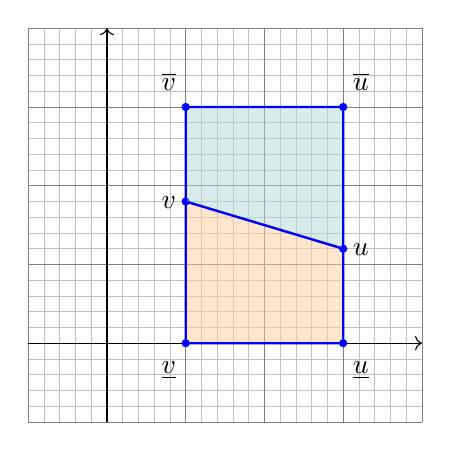
\begin{tikzpicture}[x=10mm, y=10mm, font=\mathstrut]
    \draw[style= help lines, very thin, color=lightgray, step=0.2] (-1,-1) grid (4,4);
    \draw[style= help lines, very thin, color=gray, step=1] (-1,-1) grid (4,4);
    \draw[->] (-1,0) -- (4,0); % node[below left] {$x$};
    \draw[->] (0,-1) -- (0,4); % node[below left] {$y$};
    \filldraw[draw=blue, thick, fill=orange!40, fill opacity=0.5]
    (3.0,1.2) -- (1.0,1.8) -- (1.0,0.0) -- (3.0,0.0) -- cycle;
    \draw[draw=none, fill=blue, radius=1.5pt]
    (3.0,1.2) circle node[right] {$u$}
    (1.0,1.8) circle node[left] {$v$}
    (1.0,0.0) circle node[below left] {$\underline{v}$}
    (3.0,0.0) circle node[below right] {$\underline{u}$};
    \filldraw[draw=blue, thick, fill=teal!30, fill opacity=0.5]
    (3.0,1.2) -- (3.0,3.0) -- (1.0,3.0) -- (1.0,1.8) -- cycle;
    \draw[draw=none, fill=blue, radius=1.5pt]
    (1.0,3.0) circle node[above left] {$\overline{v}$}
    (3.0,3.0) circle node[above right] {$\overline{u}$};
  \end{tikzpicture}
  \quad
  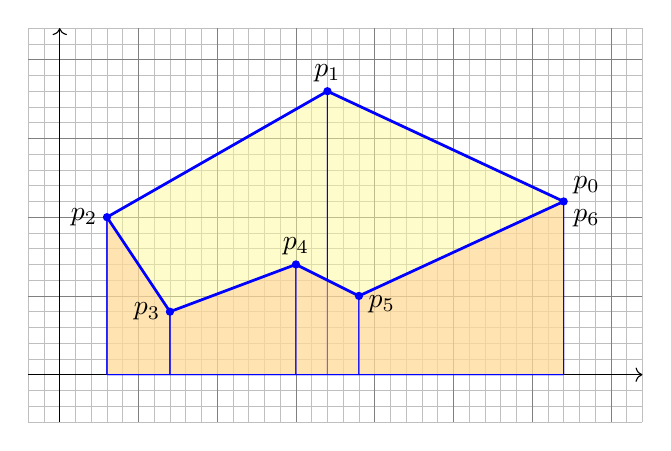
\begin{tikzpicture}[x=10mm, y=10mm, rounded corners=0.2pt]
    \draw[style= help lines, very thin, color=lightgray, step=0.2] (-0.4,-0.6) grid (7.4,4.4);
    \draw[style= help lines, very thin, color=gray, step=1.0] (-0.4,-0.6) grid (7.4,4.4);
    \draw[->] (-0.4,0.0) -- (7.4,0.0);
    \draw[->] (0.0,-0.6) -- (0.0,4.4);

    \coordinate (P0) at (6.4,2.2);
    \coordinate (P1) at (3.4,3.6);
    \coordinate (P2) at (0.6,2.0);
    \coordinate (P3) at (1.4,0.8);
    \coordinate (P4) at (3.0,1.4);
    \coordinate (P5) at (3.8,1.0);
    
    \coordinate (Q0) at (6.4,0.0);
    \coordinate (Q1) at (3.4,0.0);
    \coordinate (Q2) at (0.6,0.0);
    \coordinate (Q3) at (1.4,0.0);
    \coordinate (Q4) at (3.0,0.0);
    \coordinate (Q5) at (3.8,0.0);
    
    \draw[blue, fill=yellow!40, fill opacity=0.5]
    (Q0) -- (P0) -- (P1) -- (Q1) -- cycle;
    \draw[blue, fill=yellow!40, fill opacity=0.5]
    (Q1) -- (P1) -- (P2) -- (Q2) -- cycle;
    \draw[blue, fill=orange!40, fill opacity=0.5]
    (Q2) -- (P2) -- (P3) -- (Q3) -- cycle;
    \draw[blue, fill=orange!40, fill opacity=0.5]
    (Q3) -- (P3) -- (P4) -- (Q4) -- cycle;
    \draw[blue, fill=orange!40, fill opacity=0.5]
    (Q4) -- (P4) -- (P5) -- (Q5) -- cycle;
    \draw[blue, fill=orange!40, fill opacity=0.5]
    (Q5) -- (P5) -- (P0) -- (Q0) -- cycle;
    \draw[blue, line width=1pt]
    (P0) -- (P1) -- (P2) -- (P3) -- (P4) -- (P5) -- cycle;
    \draw[draw=none, fill=blue, radius=1.5pt]
    (P0) circle node[right, align=left] {$p_0$ \\ $p_6$}
    (P1) circle node[above] {$p_1$}
    (P2) circle node[left]  {$p_2$}
    (P3) circle node[left]  {$p_3$}
    (P4) circle node[above] {$p_4$}
    (P5) circle node[right, yshift=-3pt] {$p_{5}$};
  \end{tikzpicture}
  \caption{Area of a polygon}
\end{figure}

\begin{definition}
  Given two points $u,v \in \K^2$ we have the (oriented) area under the trapezoid,
  \[
  \area(u,v) := \frac{1}{2} (u_1 - v_1) (u_2 + v_2) .
  \]
  
  For every polygon $P = (p_0,p_1,\ldots,p_n)$ in $\K^2$
  we thus define its area to be 
  \[
  \Area(P) := \sum_{i=1}^{n} \area(p_{i-1},p_i) .
  \]
\end{definition}

\begin{remark}
  For a simply closed polygon in $\R^2$, this yields $\abs{\Area(P)} = \vol_2(B) > 0$.

  If $\Area(P) > 0$, we call our polygon $P$ \emph{positively oriented}.
  Otherwiese, if $\Area(P) < 0$, we reverse $P = (p_0,p_1,\ldots,p_n)$
  to $P' = (p_n,\ldots,p_1,p_0)$.  This does not change the curve $C$,
  but ensures that $P'$ is positively oriented.
  This will be our standard convention.
\end{remark}

This elegant definition of $\Area(P)$ clarifies
the left hand side of Pick's equation.
For the right hand side $I + J/2 - 1$
we have to define --- and then count! ---
the enclosed lattice points.
To this end we use the winding number
of our polygon $P$ around some point $q \in \K^2$.


\subsection{The euclidean angle measure}

Over $\K = \R$, we can use the \emph{euclidean angle}
$\theta = \sphericalangle(u,v)$ between vectors $u,v \in \R^2$:
For each $u \ne 0$ and $v \notin u \, \R_{\le 0}$,
there exists a unique real number $\theta \in \ee{-\pi}{\pi}$
such that rotation by $\theta$ aligns $u$ with $v$:
\[
\frac{v}{\abs{v}} = \begin{bmatrix}
  \cos\theta & -\sin\theta \\
  \sin\theta & \cos\theta
\end{bmatrix} \frac{u}{\abs{u}} .
\qquad
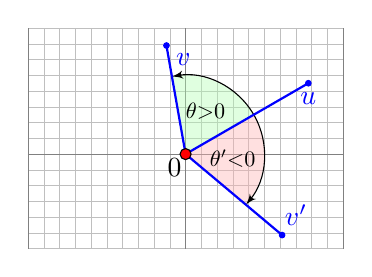
\begin{tikzpicture}[x=20mm, y=20mm, baseline={(0.2,0.0)}]
  \draw[style= help lines, very thin, color=lightgray, step=0.1] (-1.001,-0.601) grid (1.001,0.801);
  \draw[style= help lines, very thin, color=gray, step=1.0] (-1.001,-0.601) grid (1.001,0.801);
  \draw[draw=none, fill=green!30, fill opacity=0.4] (0,0) -- (30:0.5) arc (30:100:0.5) -- cycle;
  \draw[draw=black, -latex'] (30:0.5) arc (30:100:0.5);
  \draw (65:0.3) node[scale=0.8]{$\theta{>}0$};
  \draw[draw=none, fill=red!30, fill opacity=0.4] (0,0) -- (30:0.5) arc (30:-40:0.5) -- cycle;
  \draw[draw=black, -latex'] (30:0.5) arc (30:-40:0.5);
  \draw (-5:0.3) node[scale=0.8]{$\theta'{<}0$};
  \draw[draw=blue, thick] (0,0) -- (30:0.9) (0,0) -- (100:0.7) (0,0) -- (-40:0.8);
  \draw[draw=black, fill=red] (0,0) circle[radius=2pt] node[shift={(-4pt,-5pt)}] {$0$};
  \filldraw[blue, radius=1pt]
  ( 30:0.9) circle node[below] {$u$} 
  (100:0.7) circle node[right, yshift=-5pt] {$v$}
  (-40:0.8) circle node[above, xshift=+5pt] {$v'$};
\end{tikzpicture}
\]

In the controversial case $v \in u \, \R_{<0}$,
both solutions $\theta = \pm\pi$ are equally possible.
Usually this case is ignored, forbidden, or abitrated.
We democratically set $\sphericalangle(u,v) = 0$. % in this controversial case.
This choice may seem strange at first, but turns out to be advantageous.
It allows us to cover all cases uniformly,
and miraculously leads to the correct point count on the boundary.

\begin{definition}
  We define our \emph{euclidean angle measure}
  $\ang \colon \R^2 \times \R^2 \to \ee{-\sfrac{1}{2}}{+\sfrac{1}{2}}$ by
  \[
  \ang(u,v) := \begin{cases}
    \theta / 2\pi & \text{if $\abs{u} \cdot \abs{v} + u \cdot v > 0$,}
    \\ 0 & \text{if $\abs{u} \cdot \abs{v} + u \cdot v = 0$.}
  \end{cases}
  \]
  
  By summing the angles of all edges of $P$,
  we obtain the (euclidean) \emph{winding number} % of $P$ around $0$
  \[
  \Ang(P) := \sum_{i=1}^n \ang(p_{i-1},p_i) .
  \]
\end{definition}

\begin{remark}
  If our polygon $P$ is closed and $0 \notin C$, then $\Ang(P) \in \Z$
  measures how often $P$ winds around the origin.
  Likewise $\Ang(P-q) \in \Z$ measures the winding number
  around the point $q \in \R^2 \minus C$,
  where $P-q = (p_0-q,p_1-q,\ldots,p_n-q)$.

  Moreover, if $P$ is simply closed and positively oriented,
  then its Jordan decomposition $\R^2 = A \sqcup B \sqcup C$
  is characterized by the winding number:
  We have $\Ang(P-q) = 0$ for each exterior point $q \in A$
  and $\Ang(P-q) = 1$ for each interior point $q \in B$.
  We thus obtain
  \[
  I = \sum_{q \in \Z^2 \minus C} \Ang(P-q) .
  \]
  
  Our careful definition pays off for boundary points:
  We find $\Ang(P-q) = \sfrac{1}{2}$
  for $q \in \ee{p_{i-1}}{p_i}$ in the interior of any edge.
  In each vertex $p_i$, finally,
  $\Ang(P-p_i) = \alpha_i = \ang(p_{i+1}-p_i, p_{i-1}-p_i)$
  measures the enclosed angle. 
  By adding the turning angle $\beta_i = \ang(p_i-p_{i-1}, p_{i+1}-p_i)$
  each vertex point is counted by $\sfrac{1}{2}$ as well.
  The sum of all turning angles is $1$ by Hopf's umlaufsatz. % theorem.

  If $P$ is a lattice polygon, with integer vertices $v_0,\ldots,v_n \in \Z^2$, then
  \[
  J/2 - 1 = \sum_{q \in \Z^2 \cap C} \Ang(P-q) .
  \]
\end{remark}

The right hand side $I + J/2 - 1$ of Pick's equation
is defined geometrically, and usually formulated intuitively.
Any attempt to define it precisely relies on Jordan's theorem.
The winding number, as defined above, allows us to algebraically count
this as % the \emph{weighted sum of enclosed lattice points}
\[
I + J/2 - 1  = \sum_{q \in \Z^2} \Ang(P-q) .
% \Welp(P) = \sum_{q \in \Z^2} \Ang(P-q) .
\]

This reduces Pick's theorem to the following algebraic statement:

\begin{lemma}[Pick's lemma, using the euclidean angle measure] \label{lem:PickEuclidean}
  Let $p_1,\ldots,p_n=p_0 \in \Z^2$ be any sequence of integer points.
  Then the closed polygon $P = (p_0,p_1,\ldots,p_n)$ satisfies Pick's equation 
  \[
  \Area(P) = \sum_{q \in \Z^2} \Ang(P-q)
  % \Area(P) = \Welp(P)
  \]
\end{lemma}

Notice that this formulation does not require $P$ to be simple.
If $P$ is simply closed and positively oriented, 
then the right hand side equals $I + J/2 - 1$,
by Jordan and Hopf.


\subsection{The discrete angle measure}

The euclidean angle measure requires the real numbers and transcendental functions.
For computer implementation this is a burden:
\texttt{Real} is good for proofs but bad for calculation,
whereas \texttt{Float} ist good for approximations but bad for proofs.

For our purposes we prefer to work with the following \emph{discrete angle measure}.
This allows us to work over any ordered field $\K$,
for example $\Q \subseteq \K \subseteq \R$.

\begin{figure}[ht]
  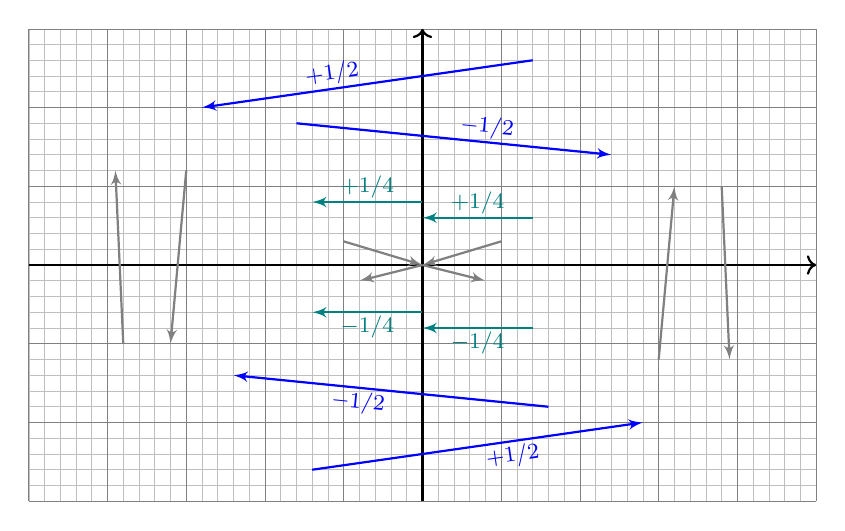
\begin{tikzpicture}[x=10mm, y=10mm, inner sep=1pt, font=\footnotesize]
    \draw[style= help lines, very thin, color=lightgray, step=0.2] (-5,-3) grid (+5,+3);
    \draw[style= help lines, very thin, color=gray, step=1] (-5,-3) grid (+5,+3);
    \draw[thick, ->] (-5,0) -- (+5,0); % node[below left] {$x$};
    \draw[thick, ->] (0,-3) -- (0,+3); % node[below left] {$y$};
    \draw[thick, blue, -latex'] (+1.4,+2.6) -- (-2.8,+2.0)
    node[pos=0.6, sloped, above]{$+1/2$};
    \draw[thick, blue, -latex'] (-1.4,-2.6) -- (+2.8,-2.0)
    node[pos=0.6, sloped, below]{$+1/2$};
    \draw[thick, blue, -latex'] (+1.6,-1.8) -- (-2.4,-1.4)
    node[pos=0.6, sloped, below]{$-1/2$};
    \draw[thick, blue, -latex'] (-1.6,+1.8) -- (+2.4,+1.4)
    node[pos=0.6, sloped, above]{$-1/2$};
    \draw[thick, teal, -latex'] (+1.4,+0.6) -- (+0.0,+0.6)
    node[pos=0.5, sloped, above]{$+1/4$};
    \draw[thick, teal, -latex'] (-0.0,+0.8) -- (-1.4,+0.8)
    node[pos=0.5, sloped, above]{$+1/4$};
    \draw[thick, teal, -latex'] (+1.4,-0.8) -- (+0.0,-0.8)
    node[pos=0.5, sloped, below]{$-1/4$};
    \draw[thick, teal, -latex'] (-0.0,-0.6) -- (-1.4,-0.6)
    node[pos=0.5, sloped, below]{$-1/4$};
    \draw[thick, black!50, -latex'] (-3.0,+1.2) -- (-3.2,-1.0);
    \draw[thick, black!50, -latex'] (-3.8,-1.0) -- (-3.9,+1.2);
    \draw[thick, black!50, -latex'] (+3.0,-1.2) -- (+3.2,+1.0);
    \draw[thick, black!50, -latex'] (+3.8,+1.0) -- (+3.9,-1.2);
    \draw[thick, black!50, -latex'] (+1.0,+0.3) -- (+0.0,+0.0);
    \draw[thick, black!50, -latex'] (+0.0,+0.0) -- (+0.8,-0.2);
    \draw[thick, black!50, -latex'] (-1.0,+0.3) -- (-0.0,+0.0);
    \draw[thick, black!50, -latex'] (-0.0,+0.0) -- (-0.8,-0.2);
  \end{tikzpicture}
  \caption{The discrete angle measure}
  \label{fig:Dang}
\end{figure}

\begin{definition}
  For the edge between any two points $u,v \in \K^2$
  we define the \emph{discrete angle measure}
  as the number of axis crossings,
  as illustrated in Figure \ref{fig:Dang}:
  \[
    \dang(u,v) :=
    \frac{1}{4} \bigabs{ \sign u_1 - \sign v_1 }
    \cdot \sign \det \begin{bmatrix} u_1 & v_1 \\ u_2 & v_2 \end{bmatrix} .
  \]

  By summing the angles of all edges of $P$,
  we obtain the (discrete) \emph{winding number} % of $P$ around $0$
  \[
  \Dang(P) := \sum_{i=1}^n \dang(p_{i-1},p_i) .
  \]
\end{definition}

If our polygon $P$ is closed and $0 \notin C$,
then we obtain $\Dang(P-q) = \Ang(P-q)$.
The summands change, but the end result is the same.
The difference is only noticable for open polygons
or boundary points $q \in C$.

% As before, if our polygon $P$ is closed,
% $\Dang(P-q) = \Ang(P-q)$ measures the winding number
% around any point $q \in \R^2 \minus C$.

The theorems of Jordan and Hopf, as stated above, continue
to hold with $\Dang(P)$ in place of $\Ang(P)$, see the Appendix.
This generalizes and simplifies! % calculations!
We can thus define the elusive right hand side $I + J/2 - 1$ of Pick's equation
by the \emph{weighted sum of enclosed lattice points}
\[
\Welp(P) := \sum_{q \in \Z^2} \Dang(P-q) .
\]

\begin{lemma}[Pick's lemma, using the discrete angle measure] \label{lem:PickDiscrete}
  Let $p_1,\ldots,p_n=p_0 \in \Z^2$ be any sequence of integer points.
  Then the closed polygon $P = (p_0,p_1,\ldots,p_n)$ satisfies Pick's equation 
  \[
  % \Area(P) = \sum_{q \in \Z^2} \Dang(P-q) .
  \Area(P) = \Welp(P) .
  \]
\end{lemma}

\begin{remark}
  At first glance this may no longer look like Pick's classical theorem.
  Admittedly, the quantity $I + J/2 - 1$ is geometrically more intuitive,
  alas notoriously vague. (``Just look!'') %  Our admirably concise
  Our formula for $\Welp(P)$ provides a precise definition,
  alas less intuitive. (``Just calculate!'')
  
  We cautiously call the above statement \emph{Pick's lemma}.
  In order to arrive at \emph{Pick's theorem},
  we have to invoke Jordan's decomposition and Hopf's umlaufsatz
  for simply closed polygonal curves.
  This bridges the gap between the algebraic lemma
  and the geometric theorem.

  Since Jordan's and Hopf's are classical theorems in their own right,
  we do not consider them as part of the \emph{proof},
  but rather use them as the foundation
  for \emph{formulating} Pick's equation. % lemma. theorem.
  This translation being achieved, we can now focus on Pick's lemma.
\end{remark}


\section{Proving Pick's lemma}

% \begin{proof}[Proof of Pick's lemma]
The sum over $q \in \Z^2$ has finite support:
We can restrict it to a sufficiently large
square box $Q = \{-r,\ldots,r\}^2 \subset \Z^2$
containing all vertices $p_1,\ldots,p_n$.
Each point $q \in \Z^2 \minus Q$ yields $\Dang(P-q) = 0$.
Using this, we rearrange the sum defining the right hand side:
\begin{alignat*}{3}
  & \Welp(P)
  % && := \sum_{q \in \Z^2} \Dang(P-q)
  && = \sum_{q \in Q} \Dang(P-q)
  && = \sum_{q \in \Z^2} \sum_{i=1}^n \dang(p_{i-1}-q, p_i-q) 
  \\ & && && = \sum_{i=1}^n
  \underbracket{ \sum_{q \in \Z^2} \dang(q_{i-1}-v, q_i-v) }_{\normalsize =: \welp(p_{i-1},p_i)}
  % \\ & && = \sum_{i=1}^n \welp(p_{i-1},p_i)
\end{alignat*}

Now both sides of Pick's equation look formally very similar:
\begin{alignat*}{3}
  & \Area(P) && = \sum_{i=1}^{n} \area(p_{i-1},p_i) ,
  \\
  & \Welp(P) && = \sum_{i=1}^n \welp(p_{i-1},p_i) .
\end{alignat*}

Here another miracle happens:
Both sums are not only equal, but termwise equal!

For any to lattice points $u,v \in Q$
in our square box $Q = \{-r,\ldots,r\}^2 \subset \Z^2$
we show that
\[
\area(u,v) = \welp(u,v) .
\]

\begin{figure}[ht]
  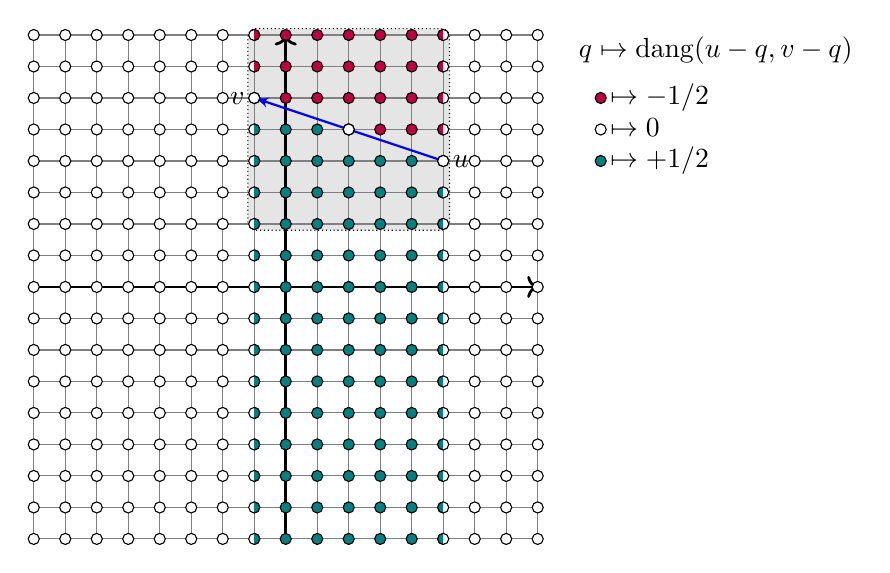
\begin{tikzpicture}[x=4mm, y=4mm, font=\mathstrut]
    \draw[draw=black, densely dotted, rounded corners=1mm, fill=black!10]
    (-1.2,+1.8) rectangle (+5.2,+8.2);
    % \draw[draw=black, rounded corners=1mm, fill=black!10]
    % (+5,+4) -- (-1,+6) -- (-1,+8) -- (+5,+8) -- cycle;
    % \draw[draw=black, rounded corners=1mm, fill=black!10]
    % (+5,-4) -- (-1,-6) -- (-1,-8) -- (+5,-8) -- cycle;
    \draw[color=black!50, step=1] (-8,-8) grid (+8,+8);
    \draw[line width=1pt, ->] (-8,0) -- (+8,0); % node[below left] {$x$};
    \draw[line width=1pt, ->] (0,-8) -- (0,+8); % node[below left] {$y$};
    
    \filldraw[draw=blue, thick, -latex'] (+5,+4) -- (-1,+6);
    \draw[draw=black, fill=white, radius=2.0pt]
    (+5,+4) circle node[right] {$u$}
    (-1,+6) circle node[left] {$v$}
    (+2,+5) circle;
    \draw (9,7.5) node[right] {$q \mapsto \dang(u-q,v-q)$};
    
    \foreach \x in {-8,-7,...,-2,6,7,...,8}{
      \foreach \y in {-8,...,8}{
        \draw[draw=black, fill=white] (\x,\y) circle[radius=2.0pt];
      }
    }
    
    \draw[draw=black, fill=white] (10,5) circle[radius=2.0pt];
    \draw (10,5) node[right] {$\mapsto 0$};
    
    
    \begin{scope}
      \foreach \y in {7,...,8}{
        \draw[draw=black, fill=white] (-1,\y) circle[radius=2.0pt];
      }
      \foreach \y in {5,...,8}{
        \draw[draw=black, fill=white] (+5,\y) circle[radius=2.0pt];
      }
      \clip (+5,+4.0) -- (+5,+8.2) -- (-1,+8.2) -- (-1,+6.0) -- cycle;
      \foreach \x in {-1,...,5}{
        \foreach \y in {-8,...,8}{
          \draw[draw=black, fill=purple] (\x,\y) circle[radius=2.0pt];
        }
      }
    \end{scope}
    
    \draw[draw=black, fill=purple] (10,6) circle[radius=2.0pt];
    \draw (10,6) node[right] {$\mapsto -1/2$};
    
    \begin{scope}
      \foreach \y in {-8,...,5}{
        \draw[draw=black, fill=white] (-1,\y) circle[radius=2.0pt];
      }
      \foreach \y in {-8,...,3}{
        \draw[draw=black, fill=white] (+5,\y) circle[radius=2.0pt];
      }
      \clip (-1,-8.2) -- (+5,-8.2) -- (+5,+4.0) -- (-1,+6.0) -- cycle;
      \foreach \x in {-1,...,5}{
        \foreach \y in {-8,...,8}{
          \draw[draw=black, fill=teal] (\x,\y) circle[radius=2.0pt];
        }
      }
    \end{scope}
    
    \draw[draw=black, fill=white]
    (-1,6) circle[radius=2.0pt]
    (+2,5) circle[radius=2.0pt]
    (+5,4) circle[radius=2.0pt];
    
    \draw[draw=black, fill=teal] (10,4) circle[radius=2.0pt];
    \draw (10,4) node[right] {$\mapsto +1/2$};
  \end{tikzpicture}
  \caption{Proving $\area(u,v) = \welp(u,v)$}
  \label{fig:AreaEqualsWelp}
\end{figure}

% We consider the edge between two integer points $u,v \in Q$.

The proof is illustrated in \autoref{fig:AreaEqualsWelp}.
The algebraic calculation proceeds as follows.
We can assume $v_1 < u_1$ and $u_2 + v_2 \ge 2$;
the other cases are symmetric.
\begin{enumerate}
\item
  For $q_1 < v_1 < u_1$ we have $\dang(u-q,v-q) = 0$.
\item
  For $q_1 > u_1 > v_1$ we have $\dang(u-q,v-q) = 0$.
\item
  The rectangle $R = \{v_1,\ldots,u_1\} \times \{u+v-r,\ldots,r\}$
  allows the involution $q \mapsto u+v-q$.
  We find $\dang(u-(u+v-q), v-(u+v-q)) = \dang(v-q,u-q) = -\dang(u-q,v-q)$.
  Thus all summands cancel pairwise,
  and we obtain $\sum_{q \in R} \dang(u-q,v-q) = 0$.
\item
  The remaining points add up to $\frac{1}{2} (u_1-v_1) (u_2+v_2) = \area(u,v)$.
\end{enumerate}

This proves $\welp(u,v) = \area(u,v)$
for any edge with end points $u,v \in Q$.
By summing over all edges of our polygon $P$,
we conclude $\Area(P) = \Welp(P)$.

% \end{proof}

\begin{remark}
  In this algebraic form, the proof is readily implemented in Lean,
  or any other proof assistant.
\end{remark}

\appendix

\section{Axiomatic angle measure}

We can use different angle measures for the theorems of
Jordan and Hopf and thus Pick.
In order to cover all cases simultaneously, 
we extract the essential properties used in the proofs:

\begin{definition}[angle measure\label{def:AngleMeasure}]
  Let $(\K,+,\cdot,\le)$ be an ordered field.
  An \emph{angle measure} is a map $\mu \colon \K^2 \times \K^2 \to \K$
  satisfying the following conditions:
  \begin{enumerate}
  \item
    Scaling: For all $u,v \in \K^2$ and $\lambda \in \K_{>0}$
    we have $\mu(u,v) = \mu(\lambda u, v) = \mu(u, \lambda v)$.
  \item
    Symmetry: $\mu(v,u) = -\mu(u,v)$ and $\mu(-u,-v) = \mu(u,v)$.
  \item
    Addition: $\mu(u,v) = \mu(u,s) + \mu(s,v)$ for $s \in [u,v]$.
  \item
    Normalisation: $\mu(e_1,e_2) = \sfrac{1}{4}$.
  \end{enumerate}
\end{definition}


\section{Jordan's decomposition for polygons}

The classical theorem, reformulated and reproven using our angle measure $\mu$.


\section{Hopf's umlaufsatz for polygons}

The classical theorem, reformulated and reproven using our angle measure $\mu$.


\section{Physical plausibility: ``water proof'' }
% \subsection{How to prove Pick's theorem?}

In every-day mathematical communication we often only sketch
the idea and appeal to some degree of informal intuition.
This is especially true for geometric statements,
like Pick's theorem, where we often heavily rely on our visual perception.
This is usually a good thing for human learning and understanding,
but it notoriously hinders any sound formalization.

We sketch such a visual proof, appealing to geometric intuition
as a counterpart to our algebraic formalization.
We then explain how the intuition can be made precise
and finally translates to our algebraic viewpoint.

\begin{figure}[ht]
  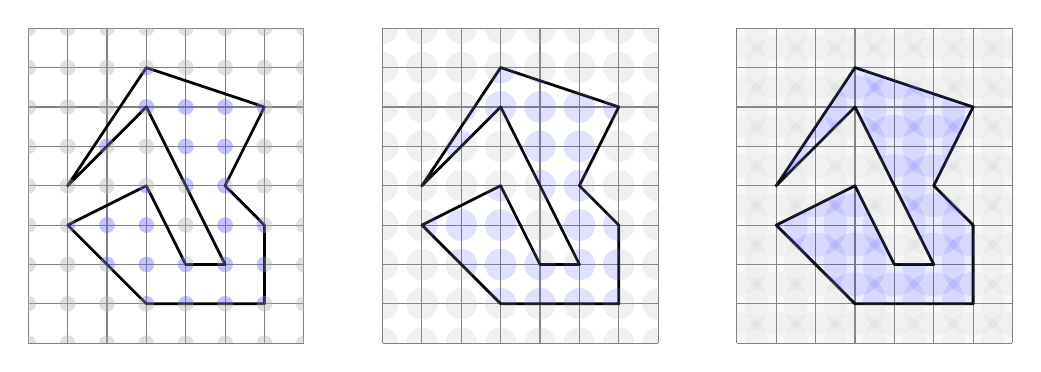
\begin{tikzpicture}[x=5mm, y=5mm, rounded corners=0.1pt]
    \begin{scope}[shift={(0,0)}]
      \draw[color=black!50, step=1] (-1,-1) grid (6,7);
      \draw[line width=1pt, black] %, fill=black!20, fill opacity=0.3]
      (0,2) -- (2,0) -- (5,0) -- (5,2) -- (4,3) -- (5,5) --
      (2,6) -- (0,3) -- (2,5) -- (4,1) -- (3,1) -- (2,3) -- cycle;
      \begin{scope}
        \clip (-1,-1) rectangle (6,7)
        (0,2) -- (2,0) -- (5,0) -- (5,2) -- (4,3) -- (5,5) --
        (2,6) -- (0,3) -- (2,5) -- (4,1) -- (3,1) -- (2,3) -- cycle;
        \foreach \x in {-1,0,...,6}{
          \foreach \y in {-1,0,...,7}{
            \draw[draw=none, fill=black!30, fill opacity=0.4] (\x,\y) circle[radius=1mm];
          }
        }
      \end{scope}
      \begin{scope}
        \clip (0,2) -- (2,0) -- (5,0) -- (5,2) -- (4,3) -- (5,5) --
        (2,6) -- (0,3) -- (2,5) -- (4,1) -- (3,1) -- (2,3) -- cycle;
        \foreach \x in {-1,0,...,6}{
          \foreach \y in {-1,0,...,7}{
            \draw[draw=none, fill=blue!60, fill opacity=0.4] (\x,\y) circle[radius=1mm];
          }
        }
      \end{scope}
    \end{scope}
    \begin{scope}[shift={(9,0)}]
      \draw[color=black!50, step=1] (-1,-1) grid (6,7);
      \draw[line width=1pt, black] %, fill=black!20, fill opacity=0.3]
      (0,2) -- (2,0) -- (5,0) -- (5,2) -- (4,3) -- (5,5) --
      (2,6) -- (0,3) -- (2,5) -- (4,1) -- (3,1) -- (2,3) -- cycle;
      \begin{scope}
        \clip (-1,-1) rectangle (6,7)
        (0,2) -- (2,0) -- (5,0) -- (5,2) -- (4,3) -- (5,5) --
        (2,6) -- (0,3) -- (2,5) -- (4,1) -- (3,1) -- (2,3) -- cycle;
        \foreach \x in {-1,0,...,6}{
          \foreach \y in {-1,0,...,7}{
            \draw[draw=none, fill=black!30, fill opacity=0.2] (\x,\y) circle[radius=2mm];
          }
        }
      \end{scope}
      \begin{scope}
        \clip (0,2) -- (2,0) -- (5,0) -- (5,2) -- (4,3) -- (5,5) --
        (2,6) -- (0,3) -- (2,5) -- (4,1) -- (3,1) -- (2,3) -- cycle;
        \foreach \x in {-1,0,...,6}{
          \foreach \y in {-1,0,...,7}{
            \draw[draw=none, fill=blue!60, fill opacity=0.2] (\x,\y) circle[radius=2mm];
          }
        }
      \end{scope}
    \end{scope}
    \begin{scope}[shift={(18,0)}]
      \draw[color=black!50, step=1] (-1,-1) grid (6,7);
      \draw[line width=1pt, black] %, fill=black!20, fill opacity=0.3]
      (0,2) -- (2,0) -- (5,0) -- (5,2) -- (4,3) -- (5,5) --
      (2,6) -- (0,3) -- (2,5) -- (4,1) -- (3,1) -- (2,3) -- cycle;
      \begin{scope}
        \clip (-1,-1) rectangle (6,7)
        (0,2) -- (2,0) -- (5,0) -- (5,2) -- (4,3) -- (5,5) --
        (2,6) -- (0,3) -- (2,5) -- (4,1) -- (3,1) -- (2,3) -- cycle;
        \foreach \x in {-1,0,...,6}{
          \foreach \y in {-1,0,...,7}{
            \draw[draw=none, fill=black!30, fill opacity=0.1] (\x,\y) circle[radius=4mm];
          }
        }
      \end{scope}
      \begin{scope}
        \clip (0,2) -- (2,0) -- (5,0) -- (5,2) -- (4,3) -- (5,5) --
        (2,6) -- (0,3) -- (2,5) -- (4,1) -- (3,1) -- (2,3) -- cycle;
        \foreach \x in {-1,0,...,6}{
          \foreach \y in {-1,0,...,7}{
            \draw[draw=none, fill=blue!80, fill opacity=0.1] (\x,\y) circle[radius=4mm];
          }
        }
      \end{scope}
    \end{scope}
  \end{tikzpicture}
  \caption{\textgreek{Πάντα ῥεῖ}, everything flows.  We let the water do the work.}
  % \caption{\textgreek{Πάντα ῥεῖ}, everything flows.  Let gravity do the work!}
  \label{fig:WaterFlow}
\end{figure}

\begin{proof}[The water proof]
  At each integer point $q \in \Z^2$ we place a unit drop of water.
  The water then flows evenly in all directions.  Finally, the plane is
  uniformly covered with water, one unit of water per unit square.
  (To ensure finiteness, we can think of periodic boundary conditions.)
  % This is a more reasonable experimental setup!

  Now consider two integer points $u,v \in \Z^2$.
  Half rotation about its center $c = (u+v)/2$
  defines the involution $\rho \colon z \mapsto u + v - z$.
  This reverses the edge and thus the flow.
  Since $\rho$ maps the lattice $\Z^2$ to itself,
  the water that flows from the point $q \in \Z^2$ over $[u,v]$ 
  is compensated by the water flowing from the point $\rho(q) \in \Z^2$ over $[u,v]$.
  The net flow over the edge $[u,v]$ is zero.
  
  This shows that the amount of water in $B$ never changes.
  At the start it is the share of drops that fall into $B$.
  At the end it equals the surface area of $B$.
  We thus obtain:
  \begin{align*}
    \vol_2(B) = I + \sum_{q \in \Z^2 \cap C} \alpha(q) / 2\pi
  \end{align*}

  Here $\alpha(q)$ is the inner angle at the boundary point $q \in C$.
  So our physical intuition, or gedankenexperiment, leads us to
  Pick's lemma \ref{lem:PickEuclidean} using the euclidean angle measure.

  We once again invoke Hopf's umlaufsatz:
  the sum of outer angles is $\sum_{q \in C} [ \pi - \alpha(q) ] = 2\pi$,
  so we arrive at Pick's theorem $\vol_2(B) = I + J/2 - 1$.
\end{proof}

% Pick's theorem can be split in two parts:
% First, the point count.
% Second, the umlaufsatz.

% The traditional way is to count each boundary point with $\sfrac{1}{2}$
% and finally add $-1$ as a correction term
% The geometric way is to count each boundary point with $\theta / 2\pi$,
% where $\theta$ is the inner angle.  For inner points this evaluates to $1$,
% for edge points to $\sfrac{1}{2}$ and for corner points to a value $\in [0,2\pi]$.
% The algebraic way is detailed below.  It is less intuitive, but much easier to compute.

\begin{remark}
  This “water proof” is a wonderful example
  of a physical plausibility argument.
  To many people is seems convincing
  because it appeals to our physical experience
  and our tried-and-tested understanding of the world.
  But is it a proof, really?
  Can we actually understand the physical world?
  It is easy to visualize, intuitively, but hard to formalize, rigorously.
\end{remark}

We can give the physical argument more mathematical substance.
%
First, we want to ensure finiteness of our experimentation table,
so instead of the entire plane $\R^2$ we consider a square $[-r,+r]^2$
with sufficiently large $r \in \N$ and periodic boundary conditions.
Geometrically, this is a flat torus $T = \R^2 / 2r\Z^2$,
and we keep all necessary symmetries: translations and reflections.

Second, we specify the properties of our idealized water drops.
For each time $t \in \ei{0}{1}$ let $\mu_t$ be a continuous probability measure,
% starting with $\mu_0$ as the Dirac measure concentrated in $0$ and
ending with the uniform (Haar) measure $\mu_1$ on $T$,
so that $4 r^2 \mu_1(B)$ is the area of our inner region. 
Now we observe the quantity 
\[
% f \colon \ei{0}{1} \to \R_{\ge0} \colon t \mapsto
f(t) := \sum_{q \in \Z^2/2r\Z^2} \mu_t(B-q) .
\]

We have $f(1) = \vol_2(B)$.
For each $t > 0$ we assume $\mu_t$ to be symmetric
with respect to $z \mapsto -z$ and uniform on its support.
Assuming that $\mu_t$ varies continuously with $t$,
the above symmetry argument suggests that $f$ is constant.
At the other end we look at the limit for $t \searrow 0$:

\begin{example}
  % In our above experiment, as illustrated in \autoref{fig:WaterFlow},
  As illustrated in \autoref{fig:WaterFlow}, for small $t$ % $0 < t \le \sfrac{1}{2}$
  we set $\supp \mu_t = D(0,t)$ to be the disc of radius $t$ around the origin $0$.
  For sufficiently small $t$ thus obtain $f(t) = \sum_{q \in \Z^2} \Ang(P-q)$.

  This recovers Pick's lemma \ref{lem:PickEuclidean}
  using the euclidean angle measure.
\end{example}

\begin{example}
  Alternatively, for small $t$ % $0 < t \le \sfrac{1}{2}$
  we consider set $\supp \mu_t = [-t^2,t^2] \times [-t,t]$
  to be a thin vertical rectangle.
  In the limit $t \searrow 0$ we thus obtain
  $f(t) \to \sum_{q \in \Z^2} \Dang(P-q)$.

  This recovers Pick's lemma \ref{lem:PickDiscrete}
  using the discrete angle measure.
\end{example}

\begin{remark}
  This tale can be recounted by replacing water with heat.
  This is appealing for a physically inclined audience
  familiar with the heat equation or diffusion.
  Moreover, this provides an explicit model of the flow
  as partial differential equations.
  Within the chosen model, we can then 
  prove that $f$ is indeed constant
  and calculate the limit for $t \searrow 0$.
  % It emphasizes superposition and the linear nature of the argument,
  % whereas the actual equations for water rather obfuscate the picture.
  % At any rate, we can choose from two versions,
  % one story each for summer and winter semesters.
\end{remark}

\begin{remark}
  Another variant is to think of reflective walls.
  Geometrically, we can take two copies of $B \cup C$
  and glue them together along their common boundary $C$.
  This produces a closed surface $S$ homeomorphic to the sphere,
  with volume $\vol_2(S) = 2 \vol_2(B)$ and Euler characteristic $\chi(S) = 2$.
  The vertices provide the curvature, as in the Gauß--Bonnet theorem.
\end{remark}

% superposition, will be used later

% Read Harrison on the tension between intuition and rigour!!!

% more rigorous proof?  Proofs from the book!
% We will not pursue this line of thought, but only give references.

%%%%%%%%%%%%%%%%%%%%%%%%%%%%%%%%%%%%%%%%%%%%%%%%%%%%%%%%%%%%%%%%%%%%%%%%%%%%%
\end{document} %%%%%%%%%%%%%%%%%%%%%%%%%%%%%%%%%%%%%%%%%%%%%%%%%%%%%%%%%%%%%%
%%%%%%%%%%%%%%%%%%%%%%%%%%%%%%%%%%%%%%%%%%%%%%%%%%%%%%%%%%%%%%%%%%%%%%%%%%%%%

%%% Local Variables: 
%%% mode: latex
%%% TeX-master: t
%%% End: 
